\renewcommand{\theequation}{\theenumi}
%\begin{enumerate}[label=\thesection.\arabic*.,ref=\thesection.\theenumi]
\begin{enumerate}[label=\arabic*.,ref=\theenumi]
\numberwithin{equation}{enumi}
\numberwithin{figure}{enumi}
\numberwithin{table}{enumi}
\numberwithin{lemma}{enumi}

\item The impulse response of a system is $h(t)=tu(t)$. For an input $u(t-1)$, the output is 
\begin{enumerate}
    \item $\dfrac{t^{2}}{2}u(t)$
    \item $\dfrac{t(t-1)}{2}u(t-1)$
    \item $\dfrac{(t-1)^{2}}{2}u(t-1)$
    \item $\dfrac{t^{2}-1}{2}u(t-1)$
\end{enumerate}
\solution
%
\begin{definition}[Laplace Transform]
It is an integral transform that converts a function of a real variable $t$ to a function of a complex variable $s$. The Laplace transform of $f(t)$ is denoted by $\mathcal{L}\cbrak{f(t)}$ or $F(s)$.
\begin{align}
    F(s)=\mathcal{L}\cbrak{f(t)}=\int_{0}^{\infty}e^{-st}f(t)dt
\end{align}
\end{definition}
\begin{remark}
Laplace transform of $f(t)=t^n,n\geq1$ is
\begin{align}
    F(s)=\mathcal{L}\cbrak{t^n}=\dfrac{n!}{s^{n+1}},s>0
    \label{ec/2013/8eq:t}
\end{align}
\end{remark}
\begin{proof}
Basis Step: $n=1$
\begin{align}
    \mathcal{L}\cbrak{t}&=\int_{0}^{\infty}e^{-st}tdt\\
    &=\sbrak{\dfrac{te^{-st}}{-s}}_{0}^{\infty}+\dfrac{1}{s}\int_{0}^{\infty}e^{-st}dt\\
    &=0+\sbrak{\dfrac{-1}{s^2}e^{-st}}_{0}^{\infty},s>0\\
    &=\dfrac{1}{s^2},s>0
\end{align}
Inductive Step:
\begin{align}
    \mathcal{L}\cbrak{t^n}&=\int_{0}^{\infty}e^{-st}t^ndt\\
    &=\sbrak{\dfrac{t^{n}e^{-st}}{-s}}_{0}^{\infty}+\dfrac{n}{s}\int_{0}^{\infty}t^{n-1}e^{-st}dt\\
    &=0+\dfrac{n}{s}\mathcal{L}\cbrak{t^{n-1}},s>0\\
    &=\dfrac{n}{s}\mathcal{L}\cbrak{t^{n-1}},s>0\label{ec/2013/8eq:e}
\end{align}
To prove that if \\eqref{ec/2003/8eq:t} holds for $n=k$, it holds for $n=k+1$. From \\eqref{ec/2003/8eq:e}
\begin{align}
    \mathcal{L}\cbrak{t^{k+1}}&=\dfrac{k+1}{s}\mathcal{L}\cbrak{t^{k}}\\
    &=\dfrac{(k+1)k!}{s(s^{k+1})}=\dfrac{(k+1)!}{s^{k+2}},s>0
\end{align}
By mathematical induction, \\eqref{ec/2003/8eq:t} is true $\forall n\geq 1$
\end{proof}
\begin{lemma}
For any real number c, 
\begin{align}
    \mathcal{L}\cbrak{u(t-c)}=\dfrac{e^{-cs}}{s}, s>0
    \label{ec/2013/8eq:u}
\end{align}
\end{lemma}
\begin{proof}
 \begin{align}
     \mathcal{L}\cbrak{u(t-c)}&=\int_{0}^{\infty}e^{-st}u(t-c)dt=\int_{c}^{\infty}e^{-st}dt\\
     &=\sbrak{-\dfrac{e^{-st}}{s}}_{c}^{\infty}=\dfrac{e^{-cs}}{s}, s>0
 \end{align}
\end{proof}
\begin{definition}[Inverse Laplace Transform]
It is the transformation of a Laplace transform into a function of time. If $F(s)=\mathcal{L}\cbrak{f(t)}$, then the Inverse laplace transform of $F(s)$ is $\mathcal{L}^{-1}\cbrak{F(s)}=f(t)$.
\end{definition}
\begin{lemma}[t-shift rule]
For any real number c,
\begin{align}
    \mathcal{L}\cbrak{u(t-c)f(t-c)}=e^{-cs}F(s)
    \label{ec/2013/8eq:uf}
\end{align}
\end{lemma}
\begin{proof}
\begin{align}
    \mathcal{L}\cbrak{u(t-c)f(t-c)}&=\int_{0}^{\infty}e^{-st}u(t-c)f(t-c)dt\\
    &=\int_{c}^{\infty}e^{-st}f(t-c)dt\\
    &=\int_{0}^{\infty}e^{-s(\tau+c)}f(\tau)d\tau \brak{t=\tau+c}\\
    &=e^{-cs}\int_{0}^{\infty}e^{-s\tau}f(\tau)d\tau\\
    &=e^{-cs}F(s)
\end{align}
\end{proof}
\begin{corollary}
\begin{align}
    \mathcal{L}^{-1}\cbrak{e^{-cs}F(s)}=u(t-c)f(t-c)
\end{align}
\end{corollary}
\begin{theorem}[Convolution theorem]
Suppose $F(s)=\mathcal{L}\cbrak{f(t)}, G(s)=\mathcal{L}\cbrak{g(t)}$ exist, then,
\begin{align}
    \mathcal{L}^{-1}\cbrak{F(s)G(s)}=f(t)*g(t)\label{ec/2013/8eq:cuf}
\end{align}
\end{theorem}
Given,
\begin{align}
    &h(t)=tu(t)\\
    &x(t)=u(t-1)
\end{align}
To find: $y(t)$. We know, 
\begin{align}
y(t)&=h(t)*x(t)\\
&=\mathcal{L}^{-1}\cbrak{H(s)X(s)}
\label{ec/2013/8eq:def}
\end{align}
From \\eqref{ec/2003/8eq:uf} and \\eqref{ec/2003/8eq:t}, 
\begin{align}
H(s)=e^{0}\mathcal{L}\cbrak{t}=\dfrac{1}{s^2}
\end{align}
From \\eqref{ec/2003/8eq:u}, 
\begin{align}
X(s)=\dfrac{e^{-s}}{s}
\end{align}
Substituting in \\eqref{ec/2003/8eq:def},
\begin{align}
y(t)=\mathcal{L}^{-1}\cbrak{\dfrac{e^{-s}}{s^3}}
% &\therefore y(t)=\begin{cases}
% 	\dfrac{(t-1)^{2}}{2}, & t \geq 1 \\~\\[-1em]
% 	0, & t < 1
% 	\end{cases}\\ 
% &\therefore y(t)=\dfrac{(t-1)^{2}}{2}u(t-1)
\end{align}
Consider 
\begin{align}
    p(t)=\dfrac{t^{2}}{2}
\end{align}
From \\eqref{ec/2003/8eq:t}
\begin{align}
    P(s)=\dfrac{2!}{2s^3}=\dfrac{1}{s^3}
\end{align}
Further, from \\eqref{ec/2003/8eq:cuf}, for $c=1$
\begin{align}
    \mathcal{L}^{-1}\cbrak{e^{-s}P(s)}&=u(t-1)p(t-1)\\
    &=u(t-1)\dfrac{(t-1)^2}{2}\\
    \therefore y(t)&=\dfrac{(t-1)^2}{2}u(t-1)
\end{align}
Option 3 is the correct answer.
\begin{align}
    h(t)&=\begin{cases}
	t, & t \geq 0 \\~\\[-1em]
	0, & t <0
	\end{cases}\\
	x(t)&=\begin{cases}
	1, & t \geq 1 \\~\\[-1em]
	0, & t <1
	\end{cases}\\
	y(t)&=\begin{cases}
	\dfrac{(t-1)^2}{2}, & t \geq 1 \\~\\[-1em]
	0, & t <1
	\end{cases}
\end{align}
See Figs. \ref{ec/2013/8plot1}, \ref{ec/2013/8plot2} and \ref{ec/2013/8plot3}.
%
\begin{figure}[!h]
 \centering
 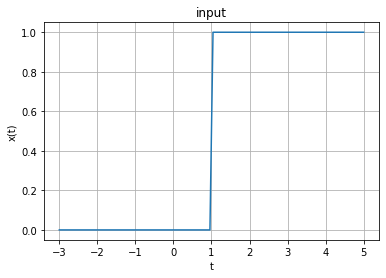
\includegraphics[width=\columnwidth]{solutions/ec/2013/8/figures/GateAssignment1(1).png}
 \caption{Plot of $x(t)$}
 \label{ec/2013/8plot1}
\end{figure}

\begin{figure}[!h]
 \centering
 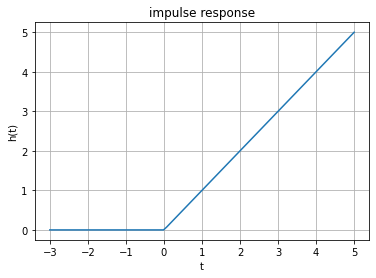
\includegraphics[width=\columnwidth]{solutions/ec/2013/8/figures/GateAssignment1(2).png}
 \caption{Plot of $h(t)$}
 \label{ec/2013/8plot2}
\end{figure}

\begin{figure}[!h]
 \centering
 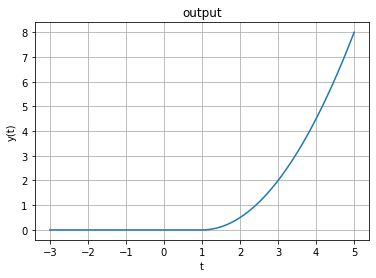
\includegraphics[width=\columnwidth]{solutions/ec/2013/8/figures/GateAssignment1(3).png}
 \caption{Plot of $y(t)$}
 \label{ec/2013/8plot3}
\end{figure}



%
\item The input $x(t)$ and output $y(t)$ of a continous time signal are related as
\begin{align}
    y(t) = \int_{t-T}^tx(u)\,du
\end{align}
The system is:
\begin{enumerate}
    \item Linear and Time-variant
    \item Linear and Time-invariant
    \item Non-Linear and Time-variant
    \item Non-Linear and Time-invariant
\end{enumerate}
\solution

\begin{definition}
We say that a system is\textbf{ linear} if and only if it follows the Principle of Superposition, i.e Law of Additivity and Law of Homogeneity.
\label{ec/2017/8/L}
\end{definition}
\begin{definition}
A system is said to be \textbf{time invariant} if the output signal does not depend on the absolute time, i.e a time delay on the input signal directly equates to the delay in the output signal.
\label{ec/2017/8/T}
\end{definition}
\begin{lemma}
The system relating the input signal $x(t$) and output signal $y(t)$, given by 
\begin{align}
     y(t) = \int_{t-T}^tx(u)\,du
\end{align}
is linear and time invariant in nature.
\end{lemma}
\begin{proof}
\begin{enumerate}
\item \textbf{\underline{Linearity and Time invariance}}\\
From \eqref{ec/2017/8/L}, we can say the system is linear if it follows both the laws of Additivity and Homogeneity.\\
\underline{Law of Additivity:}\\
Let the two input signals be $x_1(t)$ and $x_2(t)$, and their corresponding output signals be $y_1(t)$ and $y_2(t)$, then:
\begin{align}
    y_1(t) = \int_{t-T}^tx_1(u)\,du\\
    y_2(t) = \int_{t-T}^tx_2(u)\,du\\
    y_1(t) + y_2(t) = \int_{t-T}^t[x_1(u) + x_2(u)]\,du
    \label{ec/2017/8/1}
\end{align}
Now, consider the input signal of $x_1(t) + x_2(t)$, then the corresponding output signal is given by $y'(t)$:
\begin{align}
    y'(t) = \int_{t-T}^t[x_1(u) + x_2(u)]\,du
    \label{ec/2017/8/2}
\end{align}
Clearly, from \eqref{ec/2017/8/1} and \eqref{ec/2017/8/2}:
\begin{align}
    y'(t) = y_1(t) + y_2(t)
\end{align}
Thus, the Law of Additivity holds.\\

\underline{Law of Homogeneity: }\\
Consider an input signal $kx(t)$, where $k$ is any constant. Let the corresponding output be given by $y'(t)$, then:
\begin{align}
    y'(t) = \int_{t-T}^t kx(u)\,du\\
    = k\int_{t-T}^t x(u)\,du\\
     = ky(t)
     \label{ec/2017/8/3}
\end{align}
Clearly, from \eqref{ec/2017/8/3},
\begin{align}
    y'(t) = ky(t)
\end{align}
Thus, the Law of Homogeneity holds.\\

Since both the Laws hold, the system satisfies the Principle of Superposition, and is thus, a \textbf{linear system}.\\

From \eqref{ec/2017/8/T} , to check for time-invariance, we would introduce a delay of $t_0$ in the output and input signals.\\
Delay in output signal:
\begin{align}
    y(t-t_0) = \int_{t-t_0-T}^{t-t_0} x(u)\,du
    \label{ec/2017/8/4}
\end{align}
Now, we consider an input signal with a delay of $t_0$, given by $x(t-t_0)$, and let the corresponding output signal be given by $y'(t)$, then:
\begin{align}
    y'(t) = \int_{t-T}^{t} x(u-t_0)\,du
\end{align}
Substituting $a = u-t_0$:
\begin{align}
    y'(t) = \int_{t-t_0-T}^{t-t_0} x(a)\,da
    \label{ec/2017/8/5}
\end{align}
Clearly, from \eqref{ec/2017/8/4} and \eqref{ec/2017/8/5}:
\begin{align}
    y'(t) = y(t-t_0)
\end{align}
Thus, the system is \textbf{time-invariant}.\\
The correct option is \textbf{2) Linear and Time-invariant}\\


\begin{figure}[!ht]
\centering
 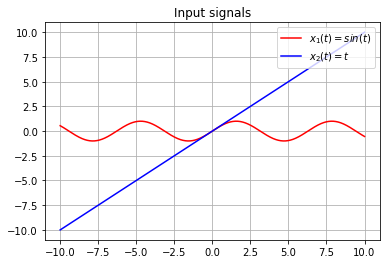
\includegraphics[width=\columnwidth]{solutions/ec/2017/8/graphs/input_signals.png}
 \caption{$x_1(t) = \sin{t}$ and $x_2(t) = t$}
 \end{figure}
\begin{figure}[!ht]
\centering
 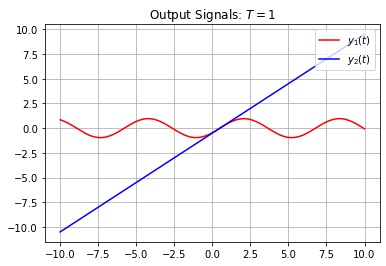
\includegraphics[width=\columnwidth]{solutions/ec/2017/8/graphs/output_signals.png}
 \caption{$y_1(t)$ and  $y_2(t)$}
 \end{figure}
 \begin{figure}[!ht]
\centering
 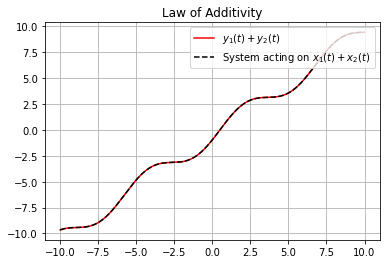
\includegraphics[width=\columnwidth]{solutions/ec/2017/8/graphs/law_of_additivity.png}
 \caption{Law of Additivity}
 \end{figure}
 \begin{figure}[!ht]
\centering
 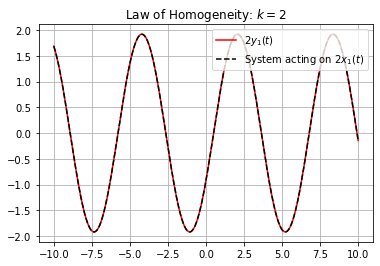
\includegraphics[width=\columnwidth]{solutions/ec/2017/8/graphs/law_of_homogeneity.png}

 \caption{Law of Homogeneity}
 \end{figure}
  \begin{figure}[!ht]
\centering
 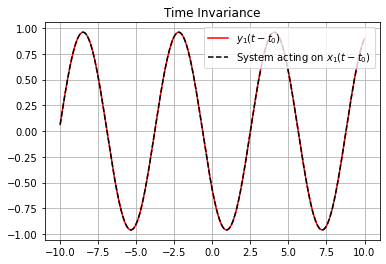
\includegraphics[width=\columnwidth]{solutions/ec/2017/8/graphs/time_invariance.png}
 \caption{Time invariance}
 \end{figure}

\item \textbf{\underline{Calculating impulse response of LTI system}}\\
Since the given system is an LTI system, it would possess an impulse response $h(t)$, which is the output of the system when the input signal is the Impulse function, given by $\delta(t)$. Thus,
\begin{align}
    h(t) = \int_{t-T}^{t} \delta(u)du
\end{align}\\
\\
The Impulse function can be loosely defined as:
\begin{align}
    \delta(t) = 
    \begin{cases}
\infty & t = 0\\
0 & otherwise
\end{cases}
and \int_{-\infty}^\infty \delta(t)dt  = 1
\end{align}
Since the Impulse function is zero everywhere aside from $t = 0$ , the non-zero value of integration is a result of $\delta(0)$. Thus, we can say $h(t)$ will be non-zero only if the limits of integration would include $t=0$, i.e:
\begin{align}
    h(t) = 
    \begin{cases}
    \int_{t-T}^{t} \delta(u)du & t-T<0 ; t>0\\
    0 & otherwise
    \end{cases}
    \end{align}
    \begin{align}
h(t) = 
    \begin{cases}
    1 & 0<t<T\\
    0 & otherwise
    \end{cases}
    \label{ec/2017/8/H}
\end{align}
\item \textbf{\underline{Expressing the impulse function in terms of $u(t)$}} \\
The unit step signal, $u(t)$, is given by:
\begin{align}
    u(t) = 
    \begin{cases}
    1 & t\geq0\\
    0 & otherwise
    \end{cases}
    \label{ec/2017/8/u(t)}
\end{align}
On time-shifting $u(t)$ by T, we get:
\begin{align}
     u(t - T) = 
    \begin{cases}
    1 & t-T\geq 0\\
    0 & otherwise
    \end{cases}
    = 
    \begin{cases}
    1 & t\geq T\\
    0 & otherwise
    \end{cases}
    \label{ec/2017/8/u(t-T)}
\end{align}
On subtracting \eqref{ec/2017/8/u(t)} and \eqref{ec/2017/8/u(t-T)}, we get our impulse response $h(t)$ in terms of the unit step signal:
\begin{align}
    h(t) = u(t) - u(t-T)
\end{align}
\item \textbf{\underline{Expressing the impulse function in terms of $rect(t)$}}\\
The unit rectangular signal, $rect(t)$ is given by:
\begin{align}
    rect(t) = 
    \begin{cases}
    1 & \frac{-1}{2} \leq t \leq \frac{1}{2} \\
    0 & otherwise
    \end{cases}
    \label{ec/2017/8/rect}
\end{align}
We can obtain the impulse response $h(t)$ in terms of $rect(t)$ using time scaling and shifting as follows:
\begin{align}
    rect\brak{\frac{t}{\tau}} = 
    \begin{cases}
    1 & \frac{-1}{2} \leq \frac{t}{\tau} \leq  \frac{1}{2}\\
    0 & otherwise
    \end{cases}
     = 
     \begin{cases}
     1 & \frac{-\tau}{2} \leq t \leq  \frac{\tau}{2}\\
    0 & otherwise
     \end{cases}
    \end{align}
    Subsituting $\tau = T$:
    \begin{align}
    rect\brak{\frac{t}{T}} = 
    \begin{cases}
    1 & \frac{-T}{2} \leq t \leq \frac{T}{2}\\
    0 & otherwise
    \end{cases}
    \end{align}
    Now, we want to right-shift the signal by $\frac{T}{2}$:
    \begin{align}
    rect\brak{\frac{1}{T}\brak{t - \frac{T}{2}}} = 
    \begin{cases}
    1 &  0 \leq t \leq T\\
    0 & otherwise
    \end{cases}
     = h(t)
\end{align}
Since the time shifting is to be performed on the variable $t$ and not $\frac{t}{T}$\\

\item 
\textbf{\underline{Calculating the Fourier Transform of $h(t)$}}\\
Let the Fourier Transform of $h(t)$ be given by $H(f)$ and of the rectangular signal, $rect(t)$ be given by $Y(f)$.
\begin{align}
    h(t) \fourier H(f)\\
    rect(t) \fourier Y(f)
    \end{align}
    Then,
    \begin{align}
    Y(f) = \int_{-\infty}^\infty rect(t)e^{-j2\pi f t}\,dt
    \label{ec/2017/8/Fourier}
\end{align}
From \eqref{ec/2017/8/rect}, we can write \eqref{ec/2017/8/Fourier} as:
\small{
\begin{align}
   Y(f) = \int_{-\infty}^\frac{-1}{2} 0\,dt + \int_{\frac{-1}{2}}^\frac{1}{2} e^{-j2\pi ft}\,dt + \int_\frac{1}{2}^\infty 0\,dt\\
    = \frac{e^{j\pi f} - e^{-j \pi f}}{j2\pi f}\\
     = \frac{2j\sin{\pi f}}{j2\pi f}\\
      = \frac{\sin (\pi f)}{\pi f}\\
       = sinc(f)
\end{align}
}
where $sinc(t)$, the sampling function is defined as:
\begin{align}
    sinc(t) = 
    \begin{cases}
    1 & t = 0\\
    \frac{\sin(\pi t)}{\pi t} & otherwise
    \end{cases}
\end{align}
Let the Fourier Transform of a signal $x(t)$ be $X(f)$.
\begin{align}
    x(t) \fourier X(f)
\end{align}
When the signal $x(t)$ is time shifted by $t_0$, the resultant Fourier Transform is given by:
\begin{align}
    x(t \pm t_0) \fourier X(f)e^{\pm j2\pi ft_0}
    \label{ec/2017/8/shift}
\end{align}
And when the signal $x(t)$ is time scaled by $\alpha$, the resulting Fourier Transform is given by:
\begin{align}
    x(\alpha t) \fourier \frac{1}{\abs{\alpha}}X\brak{\frac{f}{\alpha}}
    \label{ec/2017/8/scale}
\end{align}
Since we have already derived the Fourier Transform of $rect(t)$, we would use the properties mentioned above to find the Fourier Transform of $h(t)$:
\begin{align}
    rect(t) \fourier sinc( f)
\end{align}
Using \eqref{ec/2017/8/shift}:
\begin{align}
    rect\brak{t - \frac{T}{2}} \fourier sinc( f)e^{-j(2 \pi f)\frac{T}{2}}\\
    rect\brak{t - \frac{T}{2}} \fourier sinc( f)e^{-j \pi f T}
\end{align}
Using \eqref{ec/2017/8/scale},
\begin{align}
    rect\brak{\frac{1}{T}\brak{t - \frac{T}{2}}} \fourier \frac{1}{\frac{1}{\abs{T}}}sinc\brak{\frac{ f }{T}}e^{\frac{-j \pi f T}{T}}\\
    h(t) \fourier Tsinc\brak{\frac{ f }{T}}e^{-j\pi f}\\
    \therefore H(f)  = Tsinc\brak{\frac{ f }{T}}e^{-j\pi f}
\end{align}\\


\item \textbf{\underline{An example}}\\
Consider an input signal of $x(t) = \cos{2\pi f_0t}$. The Fourier Transform of $x(t)$ is given by:
\begin{align}
    x(t) = \cos{2\pi f_0t} \fourier \frac{1}{2}\sbrak{\delta(f - f_0) + \delta(f + f_0)}
\end{align}
using the fact that 
\begin{align}
    \cos{2\pi f_0 t} = \frac{e^{j2\pi f_0 t} + e^{-j2\pi f_0 t}}{2}
\end{align} and the Fourier Transform of $e^{\pm j2\pi f_0 t}$ is given by:
\begin{align}
    e^{\pm j2\pi  f_0 t} \fourier \delta(f \mp f_0)
    \label{ec/2017/8/FT}
\end{align}
The output signal will be given by:
\begin{align}
    y(t) = \int_{t-T}^t \cos{2\pi f_0u}\,du\\
     = \frac{1}{2\pi f_0}\sbrak{\sin{2\pi f_0t}- \sin2\pi f_0({t-T})}\\
      = \frac{\sin\pi f_0 T}{\pi f_0} \sbrak{\cos2\pi f_0 \brak{t - \frac{T}{2}}}\\
      = Tsinc(f_0 T)\cos2\pi f_0\brak{t - \frac{T}{2}}
      \label{ec/2017/8/output}
\end{align}
The Fourier transform of $\cos2\pi f_0\brak{t - \frac{T}{2}}$ can be obtained using \eqref{ec/2017/8/scale} and \eqref{ec/2017/8/shift} as follows:
\small{
\begin{align}
    \cos t = \frac{1}{2}\sbrak{e^{jt} + e^{-jt}}\\
    \cos t \fourier \frac{1}{2}\sbrak{\delta\brak{f - \frac{1}{2\pi}} + \delta\brak{f + \frac{1}{2\pi}}}\\
    \cos\brak{t - \frac{T}{2}} \fourier \frac{e^{j\pi fT}}{2}\sbrak{\delta\brak{f - \frac{1}{2\pi}} + \delta\brak{f + \frac{1}{2\pi}}} \\
    \cos2\pi f_0\brak{t - \frac{T}{2}} \fourier \frac{e^{j\pi \frac{f}{2\pi f_0}T}}{2\pi f_0}\frac{\delta(\frac{f}{2\pi f_0} - \frac{1}{2\pi}) + \delta(\frac{f}{2\pi f_0} + \frac{1}{2\pi})}{2} \\
    \cos 2\pi f_0\brak{t - \frac{T}{2}} \fourier\frac{e^{j\pi \frac{f}{2f_0}T}}{4\pi f_0}\brak{\delta\brak{\frac{f - f_0}{2\pi f_0}} + \delta\brak{\frac{f + f_0}{2\pi f_0}}}
\end{align}
}
Therefore, the Fourier Transform of the output signal $y(t)$ from \eqref{ec/2017/8/output} is given by:
 \begin{align}
     y(t) \fourier \frac{Tsinc( f_0 T)}{4\pi f_0}e^{j\pi \frac{f}{2f_0}T}\brak{\delta\brak{\frac{f - f_0}{2\pi f_0}} + \delta\brak{\frac{f + f_0}{2\pi f_0}}}\\
     y(t) \fourier ke^{j\pi \frac{f}{2f_0}T}\brak{\delta\brak{\frac{f - f_0}{2\pi f_0}} + \delta\brak{\frac{f + f_0}{2\pi f_0}}}
 \end{align}
 where $k = \frac{Tsinc( f_0T)}{4\pi f_0}$. Substituting $2\pi f_0 = 1$ and $T = 1$:
 \begin{align}
     y(t) \fourier ke^{j\pi^2f}\brak{\delta\brak{f - \frac{1}{2\pi}} + \delta\brak{f + \frac{1}{2\pi}}}\\
     y(t) \fourier ke^{j\frac{\pi}{2}}\delta\brak{f - \frac{1}{2\pi}} +ke^{j\frac{-\pi}{2}}\delta\brak{f + \frac{1}{2\pi}}
 \end{align}
 using the multiplication property of the Delta function:
 \begin{align}
     x(t)\delta(t - t_1) = x(t_1)\delta(t - t_1)
 \end{align}
 Since , $e^{j\frac{\pi}{2}} = j$ and $e^{-j\frac{\pi}{2}} = -j$, we finally get:
 \begin{align}
 y(t) \fourier kj\sbrak{\delta\brak{f - \frac{1}{2\pi}} - \delta\brak{f + \frac{1}{2\pi}}}
 \end{align}
 Clearly, the Fourier transform of $y(t)$ can be manipulated to represent a  sinusoidal wave, which is given by:
 \begin{align}
     sin(t) \fourier \frac{-j}{2}\sbrak{\delta\brak{f-\frac{1}{2\pi}} - \delta\brak{f + \frac{1}{2\pi}}}
 \end{align}
The attenuation happens for the same values of $f$, as depicted in the graphs of the Fourier Transforms given below.
\begin{figure}[!ht]
\centering
 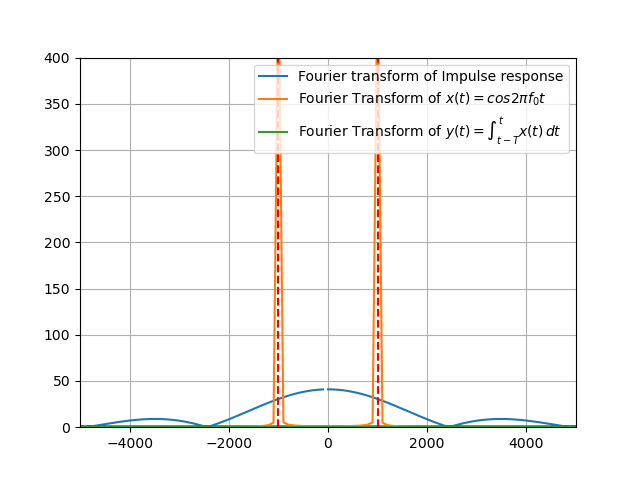
\includegraphics[width=\columnwidth]{solutions/ec/2017/8/graphs/fourier_impulse_response.png}
 \caption{Fourier Transform of Impulse response $h(t)$}
 \end{figure}
 \begin{figure}[!ht]
\centering
 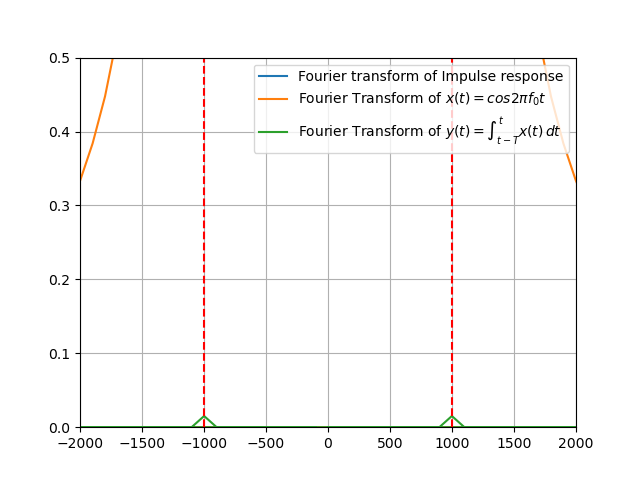
\includegraphics[width=\columnwidth]{solutions/ec/2017/8/graphs/fourier_impulse_response_zoomed.png}
 \caption{Fourier Transform of Impulse response $h(t)$ zoomed in}
 \end{figure}

\end{enumerate}
\end{proof}



\item Let the state-space representation on an LTI system be $\dot{x}(t) = Ax(t)+Bu(t)$, $y(t)=Cx(t)+du(t)$ where A,B,C are matrices,  d is a scalar, u(t) is the input to the system, and y(t) is its output. Let $B = \myvec{ 0 & 0 &  1}^\top$ and $d = 0$. Which one of the following options for A and C will ensure that the transfer function of this LTI system is 
\begin{equation}
    H(s) = \dfrac{1}{s^3+3s^2+2s+1}
\end{equation}

\begin{enumerate}[label = (\Alph*)]
    \item $A = \myvec{
     0 &  1 &  0\\ 
     0 &  0 &  1\\
    -1 & -2 & -3
    }$ and $C = \myvec{1 & 0 & 0}$
    \item $A = \myvec{
     0 &  1 &  0\\ 
     0 &  0 &  1\\
    -3 & -2 & -1
    }$ and $C = \myvec{1 & 0 & 0}$
    \item $A = \myvec{
     0 &  1 &  0\\ 
     0 &  0 &  1\\
    -1 & -2 & -3
    }$ and $C = \myvec{0 & 0 & 1}$
    \item $A = \myvec{
     0 &  1 &  0\\ 
     0 &  0 &  1\\
    -3 & -2 & -1
    }$ and $C = \myvec{0 & 0 & 1}$
    \end{enumerate}
%
\solution
From the given information, 
\begin{equation}
    \myvec{\dot{x}(t)\\y(t)} = \myvec{A & B\\C & d}\myvec{x(t)\\u(t)}
\end{equation}
%    
Taking Laplace transform on both sides,
\begin{align}
    \myvec{sX(s)\\Y(s)} &= \myvec{A & B\\ C & d}\myvec{X(s)\\U(s)}\\
    \implies sX(s) &= AX(s)+BU(s)\\
    \implies X(s) &= (sI-A)^{-1} BU(s)\\
    \implies Y(s) &= CX(s)+dU(s)\\ 
                  &= C(sI-A)^{-1} BU(s) +dU(s)
\end{align}

By definition, 
\begin{align}
    Y(s) &= H(s)U(s)\\
    \implies H(s) &= C(sI-A)^{-1} B + d\\
                  &= \dfrac{1}{s^3+3s^2+2s+1}
\end{align} 
\begin{equation}
    \implies C(sI-A)^{-1} B + d = \dfrac{1}{s^3+3s^2+2s+1}\label{ec/2019/33result}
\end{equation}

Now we cross verify the options with eq \ref{ec/2019/33result}. By using a python script, 
\begin{enumerate}[label = (\Alph*)]
    \item \begin{equation}
        C(sI-A)^{-1} B +d = \dfrac{1}{s^3+3s^2+2s+1}
    \end{equation}
    \item \begin{equation}
        C(sI-A)^{-1} B +d = \dfrac{1}{s^3+1s^2+2s+3}
    \end{equation}    
    \item \begin{equation}
        C(sI-A)^{-1} B +d = \dfrac{s^2}{s^3+3s^2+2s+1}
    \end{equation}
    \item \begin{equation}
        C(sI-A)^{-1} B +d = \dfrac{s^2}{s^3+1s^2+2s+3}
    \end{equation}
\end{enumerate}

Hence  A is the correct option.


%
\item Consider a real-valued base-band signal $x\brak{t}$, band limited to 10 kHz. The Nyquist rate for the signal $y\brak{t} = x\brak{t}x\brak{1+\frac{t}{2}}$ is
\begin{enumerate}
    \item 15 kHz
    \item 30 kHz
    \item 60 kHz
    \item 20 kHz
\end{enumerate}
\solution

\begin{definition}[Dirac-delta impulse]
\begin{align}
 \delta\brak{t}=
 \begin{cases}
 \infty , & t=0\\
 0, & otherwise
 \end{cases}
\end{align}
\end{definition}
\begin{lemma}[Shifting property of $\delta\brak{t}$]
 If $g\brak{t}$ is a continuous and finite function at $t=a$ then
 \begin{align}
     \int_{-\infty}^{\infty}\delta\brak{t-a}g\brak{t}dt=g\brak{a}
 \end{align}
 We also have
 \begin{align}
     \int_{-\infty}^{\infty}\delta\brak{t-a}\delta\brak{t-b}dt=\delta\brak{a-b}\label{translation}
 \end{align}
\end{lemma}
%%%%%%%%%
\begin{theorem}
Fourier transform of shifted impulse is the complex exponential.
\begin{align}
    G\brak{f}=\mathcal{F}\cbrak{\delta\brak{t-a}}=e^{-i2\pi fa}
\end{align}
\end{theorem}
\begin{proof}
 \begin{align}
     G\brak{f}&=\int_{-\infty}^{\infty}\delta\brak{t-a}e^{-i2\pi ft}dt\\
     &=e^{-i2\pi fa}
 \end{align}
\end{proof}
%%%%%%%%%
\begin{corollary}
Inverse Fourier Transform of the complex exponential must be the shifted impulse. So
\begin{align}
    \mathcal{F}^{-1}\cbrak{e^{-2\pi fa}}&=\int_{-\infty}^{\infty}e^{-2\pi fa}e^{i2\pi ft}df\\
    &=\int_{-\infty}^{\infty}e^{i2\pi f\brak{t-a}}df\\
    &=\int_{-\infty}^{\infty}e^{-i2\pi f\brak{t-a}}df\\
    &=\delta\brak{t-a}
\end{align}
\end{corollary}
%%%%%%%%%
\begin{theorem}
The Fourier transform of $g\brak{t}=e^{i2\pi at}$ is given by 
\begin{align}
    G\brak{f}=\mathcal{F}\cbrak{e^{i2\pi at}}=\delta\brak{f-a}
\end{align}
\begin{proof}
 \begin{align}
     G\brak{f}&=\int_{-\infty}^{\infty}e^{i2\pi at}e^{-i2\pi ft}dt\\
     &=\int_{-\infty}^{\infty}e^{i2\pi t\brak{a-f}}dt\\
     &=\delta\brak{f-a}
 \end{align}
\end{proof}
\end{theorem}
%%%%%%%%
\begin{lemma}[Linearity of Fourier Transform]
\begin{align}
    \mathcal{F}\cbrak{c_1g\brak{t}+c_2h\brak{t}}=c_1\mathcal{F}\cbrak{g\brak{t}}+c_2\mathcal{F}\cbrak{h\brak{t}}
\end{align}
\end{lemma}
%%%%%%%
\begin{lemma}\label{fre}
Let $x\brak{t}$ be a signal, its Fourier Transform  be of the form
\begin{align}
    G_x\brak{f}=c_1\delta\brak{f-a_1A}+c_2\delta\brak{f-a_2A}+...
\end{align}
where $c_i\in \mathbb{C}$ and $a_i\in \mathbb{R}$. 
Then the frequencies present in the signal are $a_jA $ where $a_j\in \mathbb{R}^{+}$
\end{lemma}
%%%%%%%
Let $x\brak{t}=\cos{\brak{2\pi At}}$, where $A=10kHz$.
\begin{align}
  \cos{\brak{2\pi At}}=\frac{e^{i2\pi At}+e^{-i2\pi At}}{2}  
\end{align}
The Fourier transform of $x\brak{t}$ 
\begin{align}
    G_x\brak{f}&=\int_{-\infty}^{\infty}\frac{e^{i2\pi At}+e^{-i2\pi At}}{2}e^{-i2\pi ft}dt\\
    &=\frac{1}{2}\sbrak{\int_{-\infty}^{\infty}e^{-i2\pi t(f-A)}dt+\int_{-\infty}^{\infty}e^{-i2\pi t(A+F)}}\\
    &=\frac{1}{2}\sbrak{\delta\brak{f-A}+\delta\brak{f+A}}
\end{align}
$\therefore$ All the energy of the sinusoidal wave is  entirely localized at the frequencies given by $|f|=A$.
\begin{align}
    y\brak{t}&=\cos{\brak{2\pi At}}\cos{\brak{2\pi A\brak{1+\frac{t}{2}}}}\\
    &=\frac{1}{2}\brak{\cos{\brak{2\pi A+3\pi At}}+\cos{\brak{2\pi A-\pi At}}}\\
    &=\frac{1}{2}\brak{\cos{\brak{3\pi At}}+\cos{\brak{\pi At}}\label{yt}}
\end{align}
Fourier Transform of $y\brak{t}$ is given by
\begin{multline}
    G_y\brak{f}=\frac{1}{4}\sbrak{\delta\brak{f-\frac{3A}{2}}+\delta\brak{f+\frac{3A}{2}}}\\+\frac{1}{4}\sbrak{\delta\brak{f-\frac{A}{2}}+\delta\brak{f+\frac{A}{2}}}
\end{multline}
From lemma $\ref{fre}$ we can conclude that the frequencies present in signal $y\brak{t}$ are $\frac{A}{2},\frac{3A}{2}$
\begin{lemma}{Multiplication property of Fourier Transform}\label{conv}
\begin{align}
    \text{If } x\brak{t} \fourier X\brak{f} \\
    y\brak{t} \fourier Y\brak{f}
\end{align}
Then
\begin{align}
   x\brak{t}y\brak{t} \fourier  X\brak{f} \ast Y\brak{f}
\end{align}
where $\ast$ represents convolution
\end{lemma}
\begin{lemma}
\begin{align}
    \delta\brak{t-t_0}\ast g\brak{t}=g\brak{t-t_0}\label{convdelta}
\end{align}
\end{lemma}
\begin{lemma}{Computing $G_y\brak{f}$ using convolution}
\begin{align}
    x\brak{t}&=\cos{\brak{2\pi At}}\\
    x\brak{t}& \fourier X_1\brak{f}=\frac{1}{2}\sbrak{\delta\brak{f-A}+\delta\brak{f+A}}\\
    x\brak{1+\frac{t}{2}}&=\cos{\brak{\pi At}}\\
    x\brak{1+\frac{t}{2}}& \fourier X_2\brak{f}=\frac{1}{2}\sbrak{\delta\brak{f-\frac{A}{2}}+\delta\brak{f+\frac{A}{2}}}
\end{align}
Using lemma $\ref{conv}$ 
\begin{align}
    G_y\brak{f}&=X_1\brak{f}\ast X_2\brak{f}\\
    &=\brak{\frac{1}{2}\sbrak{\delta\brak{f-A}+\delta\brak{f+A}}}\ast  X_2\brak{f}\\
    &=\frac{1}{2}\cbrak{\delta\brak{f-A}\ast  X_2\brak{f}+\delta\brak{f+A}\ast  X_2\brak{f}}
\end{align}
Using $\eqref{convdelta}$ 
\begin{align}
    G_y\brak{f}=\frac{1}{2}\brak{X_2\brak{f-A}+X_2\brak{f+A}}
\end{align}
\begin{multline}
    G_y\brak{f}=\frac{1}{4}\sbrak{\delta\brak{f-\frac{3A}{2}}+\delta\brak{f+\frac{3A}{2}}}\\+\frac{1}{4}\sbrak{\delta\brak{f-\frac{A}{2}}+\delta\brak{f+\frac{A}{2}}}
\end{multline}
\end{lemma}
\begin{align}
  x\brak{t}&=\cos{\brak{20k\pi t}}\\
    \text{bandwidth of } x\brak{t} &= 10 kHz\\
    x\brak{1+\frac{t}{2}} &= \cos{\brak{20k\pi+10k\pi t}}\\
    \text{bandwidth of } x\brak{1+\frac{t}{2}} &=  5 kHz\\
    \text{from \eqref{yt} } 
    y\brak{t}&= \cos{\brak{30k\pi t}}+\cos{\brak{10k\pi t}}\\
    \text{bandwidth of } y\brak{t} &= \frac{30}{2} kHz\\
    &= 15 kHz
\end{align}
\begin{align}
    \text{Nyquist rate} &= 2 \times \text{maximum frequency}\\
    &= 30 kHz
\end{align}
\begin{figure}[!h]
 \centering
 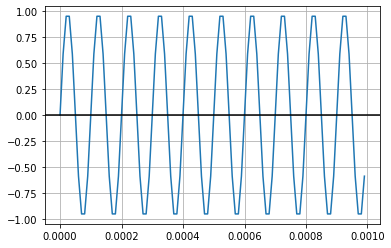
\includegraphics[width=\columnwidth]{solutions/ec/2021/4/figs/x.png}
 \caption{$x\brak{t}$:Sinusoidal signal with freq=10kHz}
\end{figure}
\begin{figure}[!h]
 \centering
 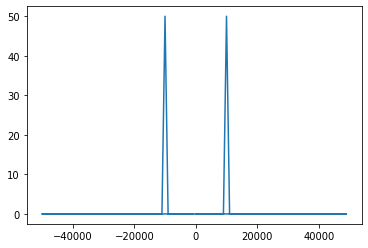
\includegraphics[width=\columnwidth]{solutions/ec/2021/4/figs/xf.png}
 \caption{DFT of $x\brak{t}$. $Bandwidth=10000$}
\end{figure}
\begin{figure}[!h]
 \centering
 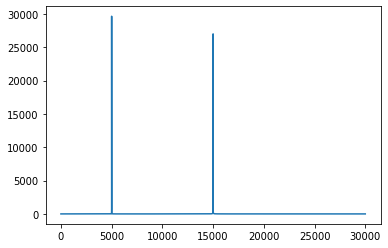
\includegraphics[width=\columnwidth]{solutions/ec/2021/4/figs/four_y.png}
 \caption{DFT of $y\brak{t}$.$Bandwidth=15000$}
\end{figure}
\begin{figure}[!h]
 \centering
 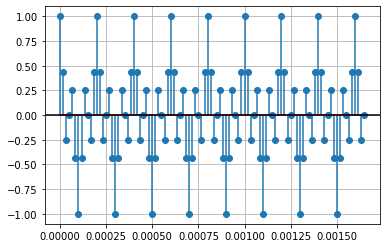
\includegraphics[width=\columnwidth]{solutions/ec/2021/4/figs/stem_y.png}
 \caption{stem plot of $y\brak{t}$ sampled at 60kHz}
\end{figure}
\begin{figure}[!h]
 \centering
 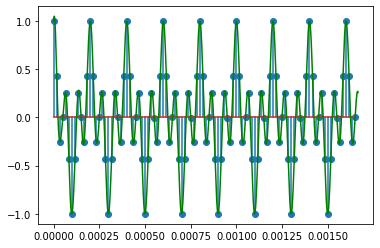
\includegraphics[width=\columnwidth]{solutions/ec/2021/4/figs/interpolation.png}
 \caption{Shannon interpolation of $y\brak{t}$}
\end{figure}





\end{enumerate}